\chapter{Entropía y energía de Gibbs de reacción}\label{ch:b2:reaction-free-energy}

Una bolsa de frío instantáneo para deportistas contiene una bolsita de agua y unas
cucharadas de nitrato de amonio. Se aprieta, la bolsita interior revienta, la sal se
disuelve y en unos segundos la bolsa está lo bastante fría para aliviar un esguince de
tobillo. La disolución absorbe calor ---es endotérmica--- y, sin embargo,
transcurre por sí sola, hasta el final. La entalpía del capítulo anterior no puede
contarlo todo: una reacción no va solo ``cuesta abajo en calor''. La magnitud que
falta es la entropía, que el segundo principio de la termodinámica, visto en física,
convierte en juez de todo cambio espontáneo. Este capítulo tabula entropías,
calcula la entropía de una reacción y combina entalpía y entropía en una sola
función, la \omterm{def:b2:reaction-free-energy:gibbs-energy}{energía de Gibbs}, cuya derivada de reacción decide el
sentido de toda reacción a temperatura y presión fijas.

\begin{recall}
De la física: el segundo principio. Todo sistema tiene una función de estado, su
entropía $S$ (extensiva); en una transformación de un sistema cerrado, $\dd S =
\delta Q/T_{\text{ext}} + \delta S_{\text{c}}$, donde la entropía creada
$\delta S_{\text{c}}$ es nula para un cambio reversible y positiva
en otro caso; para un sistema cerrado de composición fija, $\dd U = T\dd S -
p\dd V$. \Cref{ch:b2:reaction-enthalpy}: \omterm{def:b2:reaction-enthalpy:reaction-quantity}{magnitudes de reacción} $\Delta_r X =
(\partial X/\partial\xi)_{T,p}$ y \omterm{def:b2:reaction-enthalpy:standard-reaction-enthalpy}{entalpías estándar de reacción}. El volumen del
primer año enunció, como leyes ``que se deducen del segundo principio'', que una
reacción evoluciona hasta $Q = K^\circ$; este capítulo y los dos siguientes las
demuestran.
\end{recall}

\begin{omfigure}
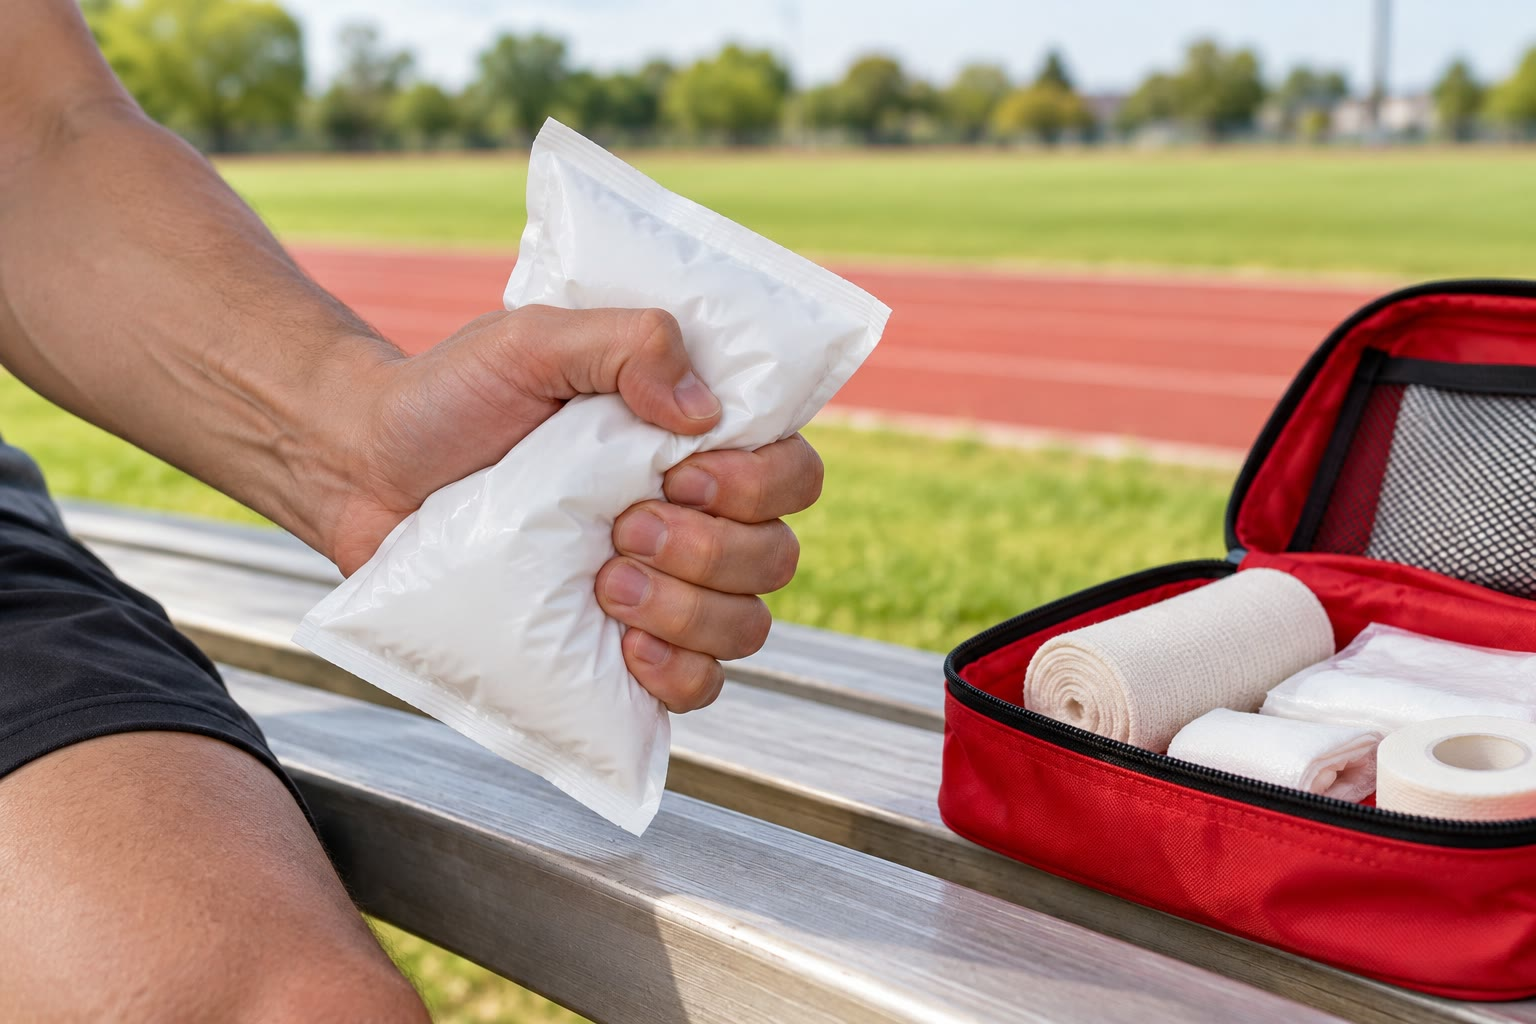
\includegraphics[width=0.55\linewidth]{images/book3/ai/b2-02-cold-pack.jpg}

{\small Una bolsa de frío: al romper su bolsita interior, el nitrato de amonio
se disuelve en el agua y la bolsa se enfría. La disolución es \omterm{def:b2:reaction-enthalpy:exothermic}{endotérmica} y
espontánea; su entropía explica por qué (\cref{ex:b2:reaction-free-energy:cold-pack}).}
\end{omfigure}

\section{Entropías estándar y tercer principio}

A diferencia de la entalpía, la entropía tiene un cero natural.

\begin{theorem}[Tercer principio de la termodinámica]\label{thm:b2:reaction-free-energy:third-law}
La entropía de un cristal puro y perfectamente ordenado tiende a cero cuando su
temperatura tiende a \qty{0}{K}.
\end{theorem}
\admitted

\begin{remark}[De dónde viene el cero]\label{rem:b2:reaction-free-energy:third-law}
Walther Nernst enunció en 1906 que las \omterm{def:b2:reaction-free-energy:reaction-entropy}{entropías de reacción} entre fases
condensadas se anulan cuando $T \to 0$; Max Planck lo precisó en el enunciado
anterior. Su origen es estadístico: la entropía cuenta las disposiciones
microscópicas compatibles con el estado de un sistema, y un cristal perfecto
a \qty{0}{K} solo tiene una. El recuento se hace en el volumen del tercer año,
con las funciones de partición.
\end{remark}

\begin{definition}[Entropía molar estándar]\label{def:b2:reaction-free-energy:standard-entropy}
La \emph{entropía molar estándar}\index{entropia molar estandar@entropía molar estándar}
$S^\circ_m(T)$ de una sustancia es la entropía de un mol de ella en su
estado estándar a la temperatura $T$, tomando como cero el del tercer principio.
A diferencia de $\Delta_f H^\circ$, es una magnitud absoluta, positiva para toda
sustancia, elementos incluidos.
\end{definition}

\begin{proposition}[Entropía absoluta a partir de las capacidades caloríficas]\label{prop:b2:reaction-free-energy:absolute-entropy}
Calentando una sustancia a presión constante $p^\circ$ desde \qty{0}{K} hasta $T$,
\[
  S^\circ_m(T) = \int_0^T\frac{C^\circ_{p,m}(T')}{T'}\,\dd T' +
  \sum_{\text{transiciones}}\frac{\Delta_{\text{trs}}H^\circ}{T_{\text{trs}}} ,
\]
tomándose la integral en cada fase sobre su intervalo de temperatura.
\end{proposition}

\begin{proof}
Calentemos la sustancia de forma reversible a presión constante: $\delta S_{\text{c}} =
0$ y $\delta Q = \dd H = C_p\,\dd T$, luego $\dd S = C_p\,\dd T/T$. En una
transición (fusión, ebullición) la temperatura se mantiene en $T_{\text{trs}}$
mientras se recibe reversiblemente el calor $\Delta_{\text{trs}}H$: la entropía
salta en $\Delta_{\text{trs}}H/T_{\text{trs}}$. Se suman las contribuciones a partir del
cero del tercer principio.
\end{proof}

\begin{omfigure}
\begin{tikzpicture}
\begin{axis}[
  width=0.8\linewidth, height=6.2cm, xmin=0, xmax=1500, ymin=0, ymax=210,
  axis x line=bottom, axis y line=left, xlabel={$T$ (K)},
  ylabel={$S^\circ_m$ del cinc (\unit{J/(K.mol)})},
  xtick={0,250,500,750,1000,1250,1500},
  tick label style={font=\small}, label style={font=\small}, clip=false]
\addplot[omDef, very thick, smooth] table[x=T, y=S] {figdata/out/bachelor-2-standard-entropy-solid.dat};
\addplot[omProp, very thick] table[x=T, y=S] {figdata/out/bachelor-2-standard-entropy-liquid.dat};
\addplot[omThm, very thick] table[x=T, y=S] {figdata/out/bachelor-2-standard-entropy-gas.dat};
\draw[densely dashed, gray] (axis cs:692.73,64.6) -- (axis cs:692.73,75.2);
\draw[densely dashed, gray] (axis cs:1180.2,91.9) -- (axis cs:1180.2,189.6);
\node[omDef, font=\small, anchor=south east] at (axis cs:600,60) {sólido};
\node[omProp, font=\small, anchor=north west] at (axis cs:850,78) {líquido};
\node[omThm, font=\small, anchor=south] at (axis cs:1350,192) {gas};
\node[font=\scriptsize, anchor=west, align=left] at (axis cs:700,110) {fusión, $+10.6$\\ a \qty{692.7}{K}};
\node[font=\scriptsize, anchor=east, align=right] at (axis cs:1170,150) {ebullición,\\ $+97.7$ a\\ \qty{1180.2}{K}};
\end{axis}
\end{tikzpicture}

{\small \omterm{def:b2:reaction-free-energy:standard-entropy}{Entropía molar estándar} del cinc a partir del cero del tercer principio. Crece
con la temperatura a medida que el metal almacena calor, y luego salta en el punto de fusión
en $\Delta_{\text{fus}}H/T_{\text{fus}}$ y, mucho más, en el punto de
ebullición en $\Delta_{\text{vap}}H/T_b$: un gas está mucho más desordenado que un
líquido.}
% ledger: s0T:Zn_crl.0, s0T:Zn_crl.298.15, s0T:Zn_cr.692, s0T:Zn_l.692, s0T:Zn_l.1180, s0T:Zn_g.1180, hT:Zn_cr.692, hT:Zn_l.692, hT:Zn_l.1180, hT:Zn_g.1180, dfh:Zn_g (curve in figdata/bachelor-2/standard-entropy.py)
\end{omfigure}

La figura da órdenes de magnitud que conviene recordar. A temperatura
ambiente un metal o un cristal duro tiene unas decenas de
\unit{J/(K.mol)}, un líquido en torno a cien, un gas de cien a trescientos;
la fusión añade un poco, la ebullición mucho. Las \omterm{def:b2:reaction-free-energy:standard-entropy}{entropías molares estándar}
que se usan en este volumen se tabulan junto con las entalpías de formación.

\section{Entropía de reacción}

\begin{definition}[Entropía de reacción]\label{def:b2:reaction-free-energy:reaction-entropy}
La \emph{entropía de reacción}\index{entropia de reaccion@entropía de reacción} es $\Delta_r S =
(\partial S/\partial\xi)_{T,p}$, y la \emph{entropía estándar de
reacción}\index{entropia estandar de reaccion@entropía estándar de reacción} es $\Delta_r S^\circ(T) =
\sum_i\nu_iS^\circ_{m,i}(T)$, en \unit{J/(K.mol)}.
\end{definition}

Como las entropías estándar son absolutas, no hace falta ninguna reacción de formación:
los elementos cuentan con sus propias entropías.

\begin{example}[Tres entropías de reacción]\label{ex:b2:reaction-free-energy:entropies}
A \qty{298.15}{K}:
\begin{itemize}
  \item \ce{CaCO3(s) -> CaO(s) + CO2(g)}: $\Delta_r S^\circ = 39.75 + 213.79 -
        92.9 = \qty{+160.6}{J/(K.mol)}$, un gas formado a partir de un sólido;
  \item \ce{N2(g) + 3H2(g) -> 2NH3(g)}: $\Delta_r S^\circ = 2(192.77) -
        191.61 - 3(130.68) = \qty{-198.1}{J/(K.mol)}$, cuatro moléculas de gas
        que se convierten en dos;
  \item \ce{N2O4(g) -> 2NO2(g)}: $\Delta_r S^\circ = 2(240.03) - 304.38 =
        \qty{+175.7}{J/(K.mol)}$.
\end{itemize}
% ledger: s0:CaCO3_cr, s0:CaO_cr, s0:CO2_g, s0:N2_g, s0:H2_g, s0:NH3_g, s0:N2O4_g, s0:NO2_g (computed in figdata/bachelor-2/thermo-data.py)
\end{example}

\begin{proposition}[El signo de una entropía de reacción]\label{prop:b2:reaction-free-energy:sign-rule}
Cuando intervienen gases, el signo de $\Delta_r S^\circ$ es en general el de
$\Delta\nu_{\text{gas}} = \sum_{\text{gases}}\nu_i$, y su magnitud es de unos
\qty{100}{} a \qty{200}{J/(K.mol)} por mol de gas formado o consumido. Cuando
$\Delta\nu_{\text{gas}} = 0$, o no interviene ningún gas, $\Delta_r S^\circ$ es
pequeña y su signo debe calcularse.
\end{proposition}

\begin{proof}[Justificación]
La entropía molar de un gas a \qty{298}{K} está entre 130 y
\qty{300}{J/(K.mol)}, la de un sólido o un líquido es de unas decenas: formar o
consumir un mol de gas domina cualquier otra contribución. Es una
regla práctica, no un teorema: la disolución de una sal, sin ningún gas, puede
cambiar la entropía en un centenar de \unit{J/(K.mol)}.
\end{proof}

\begin{method}[Prever el signo de $\Delta_r S^\circ$]\label{met:b2:reaction-free-energy:entropy-sign}
\begin{enumerate}
  \item Cuéntese $\Delta\nu_{\text{gas}}$: si no es nulo, da el
        signo.
  \item En otro caso, compárese el orden de los estados: disolver un cristal,
        fundir o romper una molécula en dos fragmentos aumentan la entropía;
        precipitar, solidificar o unir dos moléculas en una la disminuyen.
  \item Cuando la decisión importa, calcúlese $\sum_i\nu_iS^\circ_{m,i}$.
\end{enumerate}
\end{method}

El volumen del primer año encontró una consecuencia: una eliminación forma más moléculas
que una sustitución con los mismos reactivos (el alqueno, el grupo saliente
y la base protonada, frente al producto de sustitución y el grupo
saliente). Su \omterm{def:b2:reaction-free-energy:reaction-entropy}{entropía de reacción} es mayor, y el término entrópico, que crece
con la temperatura como se muestra en la sección siguiente, es la razón de que el calor favorezca
la eliminación frente a la sustitución.

\section{La energía de Gibbs}

\begin{definition}[Energía de Gibbs]\label{def:b2:reaction-free-energy:gibbs-energy}
La \emph{energía de Gibbs}\index{energia de Gibbs@energía de Gibbs} (o entalpía libre) de un sistema
es la función de estado $G = H - TS$, extensiva, en julios.
\end{definition}

\begin{definition}[Energía de Gibbs de reacción]\label{def:b2:reaction-free-energy:reaction-gibbs}
La \emph{energía de Gibbs de reacción}\index{energia de Gibbs de reaccion@energía de Gibbs de reacción} es $\Delta_r G
= (\partial G/\partial\xi)_{T,p}$, y la \emph{energía de Gibbs estándar de
reacción}\index{energia de Gibbs estandar de reaccion@energía de Gibbs estándar de reacción} es $\Delta_r G^\circ(T) =
\sum_i\nu_iG^\circ_{m,i}(T)$, ambas en \unit{kJ/mol}.
\end{definition}

\begin{proposition}[Términos entálpico y entrópico]\label{prop:b2:reaction-free-energy:g-h-s}
$\Delta_r G = \Delta_r H - T\Delta_r S$, y $\Delta_r G^\circ = \Delta_r
H^\circ - T\Delta_r S^\circ$.
\end{proposition}

\begin{proof}
Se deriva $G = H - TS$ respecto de $\xi$ a $T$ y $p$ fijas: $T$
es una constante para la derivada.
\end{proof}

\begin{proposition}[Diferencial de $G$ para un sistema en reacción]\label{prop:b2:reaction-free-energy:dG}
Para un sistema cerrado en el que tiene lugar una reacción, a $T$ y $p$
uniformes,
\[
  \dd G = V\,\dd p - S\,\dd T + \Delta_r G\,\dd\xi .
\]
\end{proposition}

\begin{proof}
$G(T, p, \xi)$ tiene la diferencial exacta $\dd G = (\partial G/\partial
T)_{p,\xi}\dd T + (\partial G/\partial p)_{T,\xi}\dd p + \Delta_r G\,\dd\xi$.
Las dos primeras derivadas parciales se toman a composición fija: son
las de un sistema cerrado de composición fija, para el que la física da
$\dd U = T\dd S - p\dd V$, de modo que $\dd G = \dd U + p\dd V + V\dd p - T\dd S
- S\dd T = V\dd p - S\dd T$. Por tanto, $(\partial G/\partial T)_{p,\xi} = -S$
y $(\partial G/\partial p)_{T,\xi} = V$.
\end{proof}

\section{El criterio de evolución}

\begin{theorem}[Criterio de evolución]\label{thm:b2:reaction-free-energy:evolution}
En un sistema cerrado mantenido a temperatura y presión constantes, que no intercambia
más trabajo que el de las fuerzas de presión, una reacción solo puede avanzar en
el sentido que hace
\[
  \Delta_r G\,\dd\xi \leq 0 ,
\]
con igualdad en el equilibrio. Si $\Delta_r G < 0$ la reacción avanza en sentido
directo, si $\Delta_r G > 0$ avanza en sentido inverso, y el sistema está en
equilibrio cuando $\Delta_r G = 0$.
\end{theorem}

\begin{proof}
Considérese un cambio infinitesimal a $T$ y $p$ uniformes, iguales a las del
entorno. El primer principio con solo trabajo de presión da $\dd U = \delta Q
- p\dd V$; el segundo da $\delta Q = T\dd S - T\delta S_{\text{c}}$. Entonces
\[
  \dd G = \dd U + p\dd V + V\dd p - T\dd S - S\dd T = -T\,\delta
  S_{\text{c}} + V\dd p - S\dd T .
\]
Comparando con la \cref{prop:b2:reaction-free-energy:dG}, a $T$ y $p$ fijas:
$\Delta_r G\,\dd\xi = -T\,\delta S_{\text{c}}$. Como $\delta S_{\text{c}}
\geq 0$, $\Delta_r G\,\dd\xi \leq 0$, y $\delta S_{\text{c}} = 0$ (un
cambio reversible, de equilibrio) exige $\Delta_r G = 0$.
\end{proof}

\begin{remark}[Lo que dice el criterio, y lo que no dice]\label{rem:b2:reaction-free-energy:criterion}
La entropía creada por una reacción a $T$ y $p$ constantes es $-\Delta_r G\,
\dd\xi/T$: la \omterm{def:b2:reaction-free-energy:gibbs-energy}{energía de Gibbs} es el segundo principio, restringido a las condiciones
del laboratorio y escrito con magnitudes del sistema solo. Dice
en qué sentido puede ir una reacción, nunca a qué velocidad: el diamante, para el que
la conversión en grafito tiene $\Delta_r G^\circ < 0$, dura para siempre en un
anillo. Y supone que no hay otro trabajo: una pila que suministra trabajo eléctrico, o un
electrolizador que lo recibe, obedece un criterio modificado
(\cref{ch:b2:cell-thermodynamics}).
\end{remark}

\begin{definition}[Exergónica y endergónica]\label{def:b2:reaction-free-energy:exergonic}
Una reacción es \emph{exergónica}\index{exergonica@exergónica} en un estado dado cuando
$\Delta_r G < 0$ y \emph{endergónica}\index{endergonica@endergónica} cuando $\Delta_r G >
0$. Con cada especie en su estado estándar, estas palabras se aplican al signo
de $\Delta_r G^\circ$.
\end{definition}

El criterio usa $\Delta_r G$, el valor en el estado real del
sistema; $\Delta_r G^\circ$ se refiere a todas las especies en su estado estándar,
que rara vez es el estado de una mezcla real. El vínculo entre ambas, a través de
la composición, es el objeto del \cref{ch:b2:chemical-potential}, y
da la ley $Q = K^\circ$ del primer año en el \cref{ch:b2:equilibrium-shifts}. Para
reacciones entre sólidos y líquidos puros, y gases a \qty{1}{bar}, las
dos coinciden.

\begin{example}[La bolsa de frío]\label{ex:b2:reaction-free-energy:cold-pack}
Para \ce{NH4NO3(s) -> NH4+(aq) + NO3-(aq)} a \qty{298.15}{K}, en estados
estándar: $\Delta_r H^\circ = -339.87 + 365.56 = \qty{+25.69}{kJ/mol}$ y
$\Delta_r S^\circ = 259.8 - 151.08 = \qty{+108.7}{J/(K.mol)}$, luego
$\Delta_r G^\circ = 25.69 - 298.15 \times 0.1087 = \qty{-6.7}{kJ/mol}$: la
disolución es \omterm{def:b2:reaction-enthalpy:exothermic}{endotérmica} y \omterm{def:b2:reaction-free-energy:exergonic}{exergónica}. Los iones, libres en el agua, están
más desordenados que en el cristal, y el término entrópico $T\Delta_r
S^\circ = \qty{32.4}{kJ/mol}$ supera el coste entálpico.
% ledger: dfh:NH4NO3_cr, s0:NH4NO3_cr, dfh:NH4NO3_ai, s0:NH4NO3_ai (computed in figdata/bachelor-2/thermo-data.py)
\end{example}

\begin{history}[Josiah Willard Gibbs]
\begin{minipage}[t]{0.2\linewidth}\vspace{0pt}
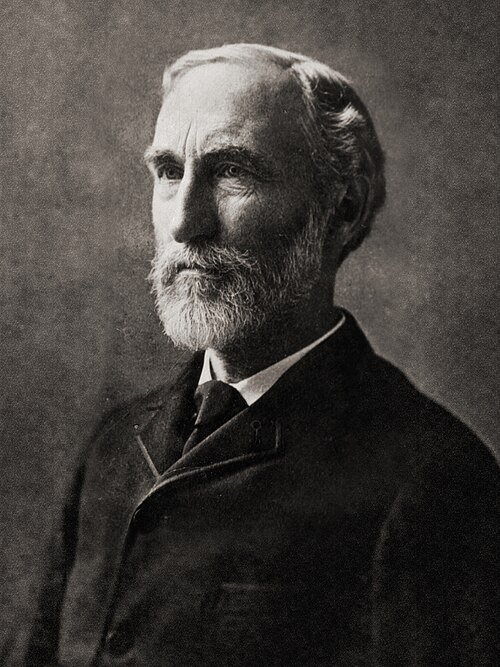
\includegraphics[width=\linewidth]{images/book3/gibbs.jpg}
\end{minipage}\hfill
\begin{minipage}[t]{0.76\linewidth}\vspace{0pt}
Josiah Willard Gibbs (1839--1903), profesor de física matemática en
Yale, publicó entre 1876 y 1878 \emph{On the Equilibrium of
Heterogeneous Substances}, unas trescientas páginas en las actas de
una pequeña academia, donde aparecen ya la energía libre, el potencial químico y la
regla de las fases de los capítulos siguientes. Pocos químicos lo leyeron hasta que
se tradujo en la década de 1890. (Fotografía: dominio público, Wikimedia
Commons.)
\end{minipage}
\end{history}

\section{Energías de Gibbs estándar de reacción y temperatura}

\begin{definition}[Aproximación de Ellingham]\label{def:b2:reaction-free-energy:ellingham-approximation}
La \emph{aproximación de Ellingham}\index{aproximacion de Ellingham@aproximación de Ellingham} considera
$\Delta_r H^\circ$ y $\Delta_r S^\circ$ independientes de la temperatura
en un intervalo que no contiene ningún cambio de estado. Entonces $\Delta_r G^\circ(T)
= \Delta_r H^\circ - T\Delta_r S^\circ$ es una recta en $T$, de pendiente
$-\Delta_r S^\circ$.
\end{definition}

\begin{proposition}[Derivadas respecto de la temperatura]\label{prop:b2:reaction-free-energy:gibbs-helmholtz}
\[
  \frac{\dd\Delta_r G^\circ}{\dd T} = -\Delta_r S^\circ, \qquad
  \frac{\dd}{\dd T}\!\left(\frac{\Delta_r G^\circ}{T}\right) =
  -\frac{\Delta_r H^\circ}{T^2}\ \ \text{(Gibbs--Helmholtz)}, \qquad
  \frac{\dd\Delta_r S^\circ}{\dd T} = \frac{\Delta_r C^\circ_p}{T}.
\]
En particular, la \omterm{def:b2:reaction-free-energy:ellingham-approximation}{aproximación de Ellingham} se cumple cuando $\Delta_r C^\circ_p$
es pequeña.
\end{proposition}

\begin{proof}
Con cada especie en su estado estándar, $G^\circ(T, \xi)$ cumple $(\partial
G^\circ/\partial T)_\xi = -S^\circ$ (\cref{prop:b2:reaction-free-energy:dG}).
Por el teorema de Schwarz,
\[
  \frac{\dd\Delta_r G^\circ}{\dd T} = \partial_\xi\partial_T G^\circ =
  -\partial_\xi S^\circ = -\Delta_r S^\circ .
\] Después, $\frac{\dd}{\dd
T}(\Delta_r G^\circ/T) = \frac{-T\Delta_r S^\circ - \Delta_r G^\circ}{T^2} =
-\frac{\Delta_r H^\circ}{T^2}$. Por último, $\dd S^\circ_m = C^\circ_{p,m}\,\dd
T/T$ para cada especie (\cref{prop:b2:reaction-free-energy:absolute-entropy}),
y la misma combinación da la última relación. Si $\Delta_r C^\circ_p$ es
pequeña, $\Delta_r H^\circ$ (Kirchhoff) y $\Delta_r S^\circ$ apenas varían.
\end{proof}

\begin{definition}[Temperatura de inversión]\label{def:b2:reaction-free-energy:inversion-temperature}
Cuando $\Delta_r H^\circ$ y $\Delta_r S^\circ$ tienen el mismo signo, la
\emph{temperatura de inversión}\index{temperatura de inversion@temperatura de inversión} de la reacción es
la temperatura a la que $\Delta_r G^\circ$ cambia de signo; en la \omterm{def:b2:reaction-free-energy:ellingham-approximation}{aproximación
de Ellingham}, $T_i = \Delta_r H^\circ/\Delta_r S^\circ$.
\end{definition}

\begin{omfigure}
\begin{tikzpicture}
\begin{axis}[
  width=0.72\linewidth, height=5.6cm, xmin=0, xmax=1600, ymin=0, ymax=260,
  axis x line=bottom, axis y line=left, xlabel={$T$ (K)}, ylabel={\unit{kJ/mol}},
  tick label style={font=\small}, label style={font=\small}, clip=false]
\addplot[omThm, very thick] table[x=T, y=DrH] {figdata/out/bachelor-2-thermo-data-calcite.dat};
\addplot[omDef, very thick] table[x=T, y=TDrS] {figdata/out/bachelor-2-thermo-data-calcite.dat};
\node[omThm, anchor=south west, font=\small] at (axis cs:60,180) {$\Delta_r H^\circ = 178.3$};
\node[omDef, anchor=west, font=\small] at (axis cs:1600,257) {$T\Delta_r S^\circ$};
\draw[dotted] (axis cs:1110,0) -- (axis cs:1110,178.3);
\node[anchor=south west, font=\small] at (axis cs:1120,8) {$T_i = \qty{1110}{K}$};
\node[font=\scriptsize, align=center] at (axis cs:600,140) {$\Delta_r G^\circ > 0$:\\ calcita estable};
\node[font=\scriptsize, align=center] at (axis cs:1470,206) {$\Delta_r G^\circ < 0$};
\end{axis}
\end{tikzpicture}

{\small Los términos entálpico y entrópico de \ce{CaCO3(s) -> CaO(s) + CO2(g)}
en la \omterm{def:b2:reaction-free-energy:ellingham-approximation}{aproximación de Ellingham}. Por debajo de la \omterm{def:b2:reaction-free-energy:inversion-temperature}{temperatura de inversión} gana el
coste entálpico y la caliza es estable bajo \qty{1}{bar} de dióxido de
carbono; por encima gana el término entrópico y la caliza se descompone.}
% ledger: dfh:CaCO3_cr, dfh:CaO_cr, dfh:CO2, s0:CaCO3_cr, s0:CaO_cr, s0:CO2_g (computed in figdata/bachelor-2/thermo-data.py)
\end{omfigure}

\begin{omfigure}
\begin{tikzpicture}[font=\small]
  \draw[thick] (0,0) rectangle (8,4);
  \draw[thick] (4,0) -- (4,4) (0,2) -- (8,2);
  \node[above] at (2,4) {$\Delta_r H^\circ < 0$};
  \node[above] at (6,4) {$\Delta_r H^\circ > 0$};
  \node[left] at (0,3) {$\Delta_r S^\circ > 0$};
  \node[left] at (0,1) {$\Delta_r S^\circ < 0$};
  \node[align=center, omDef] at (2,3) {exergónica\\ a cualquier $T$};
  \node[align=center, omProp] at (6,3) {exergónica\\ por encima de $T_i$};
  \node[align=center, omProp] at (2,1) {exergónica\\ por debajo de $T_i$};
  \node[align=center, omThm] at (6,1) {endergónica\\ a cualquier $T$};
\end{tikzpicture}

{\small Los cuatro casos de $\Delta_r G^\circ = \Delta_r H^\circ - T\Delta_r
S^\circ$ (\omterm{def:b2:reaction-free-energy:ellingham-approximation}{aproximación de Ellingham}). Las combustiones están en la casilla superior izquierda;
la descomposición de la caliza y la bolsa de frío, en la superior derecha; la
síntesis del amoníaco, en la inferior izquierda.}
\end{omfigure}

\begin{method}[Una energía de Gibbs estándar de reacción a la temperatura $T$]\label{met:b2:reaction-free-energy:delta-g-standard}
\begin{enumerate}
  \item Con las tablas a \qty{298.15}{K}, calcúlense $\Delta_r H^\circ$ y
        $\Delta_r S^\circ$.
  \item Compruébese que ninguna especie cambia de estado entre \qty{298}{K} y $T$;
        en caso contrario, añádase la transición (entalpía y entropía) o pártase
        del nuevo estado.
  \item En la \omterm{def:b2:reaction-free-energy:ellingham-approximation}{aproximación de Ellingham}, $\Delta_r G^\circ(T) = \Delta_r H^\circ
        - T\Delta_r S^\circ$.
  \item Cuando $\Delta_r C^\circ_p$ no es pequeña o el intervalo es largo,
        úsense directamente valores tabulados de $\Delta_f G^\circ(T)$.
\end{enumerate}
\end{method}

\begin{example}[Dos pruebas de la aproximación]\label{ex:b2:reaction-free-energy:tests}
Para la caliza, $\Delta_r C^\circ_p = 42.80 + 37.13 - 81.88 =
\qty{-2.0}{J/(K.mol)}$: la aproximación es excelente, y $\Delta_r
G^\circ = 178.3 - T \times 0.1606$ da $T_i = \qty{1110}{K}$. Para el amoníaco,
$\Delta_r G^\circ(700) \approx -91.9 + 700 \times 0.1981 =
\qty{+46.8}{kJ/mol}$, mientras que las tablas dan $2\Delta_f G^\circ(\ce{NH3}, 700) =
\qty{+54.4}{kJ/mol}$: aquí $\Delta_r C^\circ_p = \qty{-44}{J/(K.mol)}$ y
el error es de \qty{8}{kJ/mol}, un factor 4 en la constante de equilibrio a
esa temperatura.
% ledger: cp:CaO_cr.298, cp:CO2_g.298, cp:CaCO3_cr.298, janafG:NH3.700 (computed in figdata/bachelor-2/thermo-data.py)
\end{example}

\section{Ejercicios}

\begin{exercise}[$\star$]\label{exo:b2:reaction-free-energy:1}
Prevéase el signo de $\Delta_r S^\circ$ para: (a) \ce{2H2(g) + O2(g) -> 2H2O(l)};
(b) \ce{CaCO3(s) -> CaO(s) + CO2(g)}; (c) \ce{N2O4(g) -> 2NO2(g)};
(d) \ce{Ag+(aq) + Cl-(aq) -> AgCl(s)}; (e) \ce{H2O(s) -> H2O(l)};
(f) \ce{H2(g) + Cl2(g) -> 2HCl(g)}.
\end{exercise}

\begin{exercise}[$\star$]\label{exo:b2:reaction-free-energy:2}
Calcúlense $\Delta_r S^\circ$ y $\Delta_r G^\circ$ a \qty{298.15}{K} para la
síntesis del amoníaco, \ce{N2(g) + 3H2(g) -> 2NH3(g)}, con $\Delta_r
H^\circ = \qty{-91.9}{kJ/mol}$ y las entropías del capítulo. ¿Es
\omterm{def:b2:reaction-free-energy:exergonic}{exergónica}?
\end{exercise}

\begin{exercise}[$\star$]\label{exo:b2:reaction-free-energy:3}
Calcúlese $\Delta_r G^\circ(\qty{298.15}{K})$ de \ce{H2(g) + 1/2O2(g) ->
H2O(l)} a partir de $\Delta_f H^\circ(\ce{H2O}, \text{l}) = \qty{-285.83}{kJ/mol}$
y de las entropías estándar \ce{H2(g)} 130.68, \ce{O2(g)} 205.15 y
\ce{H2O(l)} \qty{69.95}{J/(K.mol)}. ¿Por qué este valor es la \omterm{def:b2:reaction-free-energy:gibbs-energy}{energía de Gibbs}
estándar de formación del agua líquida?
% ledger: dfh:H2O-l, s0:H2_g, s0:O2_g, s0:H2O_l
\end{exercise}

\begin{exercise}[$\star$]\label{exo:b2:reaction-free-energy:4}
Léanse en la figura de la entropía del cinc su \omterm{def:b2:reaction-free-energy:standard-entropy}{entropía molar estándar} a
\qty{298}{K} y a \qty{1000}{K}, y sus saltos en los puntos de fusión y de
ebullición. Dedúzcanse sus entalpías de fusión y de vaporización.
\end{exercise}

\begin{exercise}[$\star\star$]\label{exo:b2:reaction-free-energy:5}
Para \ce{H2O(l) -> H2O(g)} a \qty{298.15}{K}, calcúlense $\Delta_r H^\circ$,
$\Delta_r S^\circ$ y $\Delta_r G^\circ$ con las tablas del capítulo.
Explíquese por qué $\Delta_r S^\circ \neq \Delta_r H^\circ/T$ a \qty{298}{K} y qué
significa un $\Delta_r G^\circ$ positivo, y estímese con la \omterm{def:b2:reaction-free-energy:ellingham-approximation}{aproximación de
Ellingham} la temperatura a la que el agua líquida y su vapor a
\qty{1}{bar} están en equilibrio. Compárese con el punto de ebullición.
\end{exercise}

\begin{exercise}[$\star\star$]\label{exo:b2:reaction-free-energy:6}
Para \ce{N2O4(g) -> 2NO2(g)}, $\Delta_r H^\circ = \qty{57.1}{kJ/mol}$ y
$\Delta_r S^\circ = \qty{175.7}{J/(K.mol)}$. Calcúlese la \omterm{def:b2:reaction-free-energy:inversion-temperature}{temperatura de
inversión}, y explíquese por qué un tubo sellado del gas pardo \ce{NO2} palidece
cuando se enfría en hielo.
\end{exercise}

\begin{exercise}[$\star\star$]\label{exo:b2:reaction-free-energy:7}
Una reacción tiene $\Delta_r G^\circ = \qty{-12.0}{kJ/mol}$ a \qty{300}{K}
y $\qty{-4.0}{kJ/mol}$ a \qty{400}{K}. En la \omterm{def:b2:reaction-free-energy:ellingham-approximation}{aproximación de Ellingham},
hállense $\Delta_r H^\circ$ y $\Delta_r S^\circ$, y compruébese la
relación de Gibbs--Helmholtz.
\end{exercise}

\begin{exercise}[$\star\star$]\label{exo:b2:reaction-free-energy:8}
Calcúlese $\Delta_r G^\circ$ de la formación del metano, \ce{C(s) + 2H2(g) ->
CH4(g)}, a \qty{298.15}{K}, a partir de $\Delta_f H^\circ = \qty{-74.87}{kJ/mol}$
y de las entropías \ce{C} (grafito) 5.74, \ce{H2} 130.68 y \ce{CH4}
\qty{186.25}{J/(K.mol)}. ¿Por encima de qué temperatura el metano se vuelve
inestable respecto de sus elementos a la presión estándar?
% ledger: dfh:CH4_g, s0:C_gr, s0:H2_g, s0:CH4_g
\end{exercise}

\begin{exercise}[$\star\star$]\label{exo:b2:reaction-free-energy:9}
Un halogenoalcano reacciona con una base por sustitución o por eliminación. Escríbanse
ambas reacciones para el 2-bromopropano y el ion hidróxido. Con $\Delta_r
H^\circ(\text{eliminación}) - \Delta_r H^\circ(\text{sustitución}) =
\qty{+40}{kJ/mol}$ y $\Delta_r S^\circ(\text{eliminación}) - \Delta_r
S^\circ(\text{sustitución}) = \qty{+90}{J/(K.mol)}$ (órdenes de magnitud),
hállese por encima de qué temperatura la eliminación pasa a ser la más \omterm{def:b2:reaction-free-energy:exergonic}{exergónica} de
las dos, y explíquese el papel del número de moléculas.
\end{exercise}

\begin{exercise}[$\star\star\star$]\label{exo:b2:reaction-free-energy:10}
El monóxido de carbono cristalino no alcanza entropía nula a \qty{0}{K}: cada
molécula puede situarse como CO o como OC casi al azar, pues las dos orientaciones tienen
casi la misma energía. Admitiendo la fórmula de Boltzmann $S = k_B\ln W$, donde
$W$ es el número de disposiciones (que se cuentan en el volumen del tercer año), calcúlese
la entropía molar residual. ¿Por qué no se aplica el tercer principio a este
cristal?
\end{exercise}

\begin{exercise}[$\star\star\star$]\label{exo:b2:reaction-free-energy:11}
Demuéstrese que, si $\Delta_r C^\circ_p$ es una constante $c$,
$\Delta_r S^\circ(T) = \Delta_r S^\circ(T_0) + c\ln(T/T_0)$ y
$\Delta_r G^\circ(T) = \Delta_r H^\circ(T_0) - T\Delta_r S^\circ(T_0) +
c\,[T - T_0 - T\ln(T/T_0)]$. Aplíquese a la caliza ($c =
\qty{-2.0}{J/(K.mol)}$) a \qty{1100}{K}, y mídase el error de la
\omterm{def:b2:reaction-free-energy:ellingham-approximation}{aproximación de Ellingham}.
\end{exercise}

\begin{exercise}[$\star\star\star$]\label{exo:b2:reaction-free-energy:12}
El titanio se obtiene de su óxido, el rutilo, a través de su cloruro. (a) Calcúlense
$\Delta_r H^\circ$ y $\Delta_r S^\circ$ a \qty{298}{K} de \ce{TiO2(s) +
2Cl2(g) -> TiCl4(g) + O2(g)}, con \ce{TiO2} ($-944.0$ \unit{kJ/mol},
\qty{50.62}{J/(K.mol)}) y \ce{TiCl4(g)} ($-763.2$, 353.2), y su
$\Delta_r G^\circ$ a \qty{1000}{K} en la \omterm{def:b2:reaction-free-energy:ellingham-approximation}{aproximación de Ellingham}.
(b) Se añade carbono: \ce{C(s) + O2(g) -> CO2(g)}, $\Delta_r H^\circ =
\qty{-393.5}{kJ/mol}$, $\Delta_r S^\circ = \qty{+2.9}{J/(K.mol)}$. Calcúlese
$\Delta_r G^\circ(\qty{1000}{K})$ de la suma de las dos reacciones y
explíquese cómo la segunda arrastra a la primera.
% ledger: dfh:TiO2_cr, s0:TiO2_cr, dfh:TiCl4_g, s0:TiCl4_g, s0:Cl2_g, s0:O2_g, s0:C_gr, s0:CO2_g
\end{exercise}

\section{Problema: el horno de cal}

\begin{problem}[{Problema de fin de semana --- la entropía y la entalpía de una
descomposición, su energía de Gibbs frente a la temperatura, el criterio de
evolución en un horno y la energía y el dióxido de carbono de una tonelada de
cal}]
\label{pb:b2:reaction-free-energy:1}
La cal, \ce{CaO}, se obtiene calentando caliza, \ce{CaCO3}, en un horno. Datos a
\qty{298.15}{K}: $\Delta_f H^\circ$ (\unit{kJ/mol}) \ce{CaCO3(s)}
$-1206.92$, \ce{CaO(s)} $-635.09$, \ce{CO2(g)} $-393.51$; $S^\circ_m$
(\unit{J/(K.mol)}) 92.9, 39.75, 213.79; $C^\circ_{p,m}$ (\unit{J/(K.mol)})
81.88, 42.80, 37.13. Masas molares: \ce{CaO} \qty{56.08}{g/mol}, \ce{CO2}
\qty{44.01}{g/mol}, \ce{CH4} \qty{16.04}{g/mol}; combustión del metano,
con el agua como vapor, $\Delta_r H^\circ = \qty{-802.3}{kJ/mol}$.
% ledger: dfh:CaCO3_cr, dfh:CaO_cr, dfh:CO2, s0:CaCO3_cr, s0:CaO_cr, s0:CO2_g, cp:CaCO3_cr.298, cp:CaO_cr.298, cp:CO2_g.298

\medskip
\noindent\textbf{Parte I --- A temperatura ambiente.}
\begin{enumerate}
  \item Escríbase la descomposición de la caliza.
  \item Calcúlese $\Delta_r H^\circ(\qty{298}{K})$. ¿Es \omterm{def:b2:reaction-enthalpy:exothermic}{exotérmica} la reacción?
  \item Calcúlese $\Delta_r S^\circ(\qty{298}{K})$ y explíquese su signo.
  \item Calcúlese $\Delta_r G^\circ(\qty{298}{K})$.
  \item ¿Es estable la caliza a temperatura ambiente bajo \qty{1}{bar} de
        dióxido de carbono? ¿Por qué perduran los acantilados calizos?
  \item Calcúlese $\Delta_r C^\circ_p$ y dígase qué implica para la
        dependencia de $\Delta_r H^\circ$ y $\Delta_r S^\circ$ con la temperatura.
\end{enumerate}

\medskip
\noindent\textbf{Parte II --- El calentamiento.}
\begin{enumerate}[resume]
  \item Escríbase $\Delta_r G^\circ(T)$ en la \omterm{def:b2:reaction-free-energy:ellingham-approximation}{aproximación de Ellingham}.
  \item Calcúlese a \qty{1000}{K} y a \qty{1300}{K}.
  \item Calcúlese la \omterm{def:b2:reaction-free-energy:inversion-temperature}{temperatura de inversión} $T_i$.
  \item Compruébese la relación de Gibbs--Helmholtz sobre esta expresión.
  \item Estímense, con la fórmula del \cref{exo:b2:reaction-free-energy:11},
        la variación de $\Delta_r G^\circ$ en $T_i$ debida a
        $\Delta_r C^\circ_p$ y el desplazamiento de $T_i$ que resulta.
\end{enumerate}

\medskip
\noindent\textbf{Parte III --- El horno.}
En esta parte el dióxido de carbono sobre los sólidos está a \qty{1}{bar}, de modo
que $\Delta_r G = \Delta_r G^\circ$.
\begin{enumerate}[resume]
  \item ¿Qué dice el criterio de evolución a \qty{1000}{K}? ¿Y a
        \qty{1300}{K}?
  \item ¿Qué le ocurre a una mezcla de cal y dióxido de carbono a
        \qty{1}{bar} enfriada por debajo de $T_i$?
  \item ¿Cuánta entropía se crea por mol de caliza descompuesto a
        \qty{1300}{K}?
  \item Los hornos están barridos por los gases de combustión, más pobres en dióxido de carbono.
        Aventúrese, antes del capítulo siguiente, si esto favorece la
        descomposición.
\end{enumerate}

\medskip
\noindent\textbf{Parte IV --- Una tonelada de cal.}
\begin{enumerate}[resume]
  \item Calcúlese la cantidad de cal que hay en una tonelada.
  \item Calcúlese el calor absorbido por la reacción por tonelada de cal
        (tómese $\Delta_r H^\circ$ como constante).
  \item Calcúlese la masa de dióxido de carbono liberada por la caliza por
        tonelada de cal.
  \item El calor procede de la combustión de metano con un rendimiento útil del
        50\,\%. Calcúlese la masa de metano quemada por tonelada de cal.
  \item Calcúlese el dióxido de carbono procedente de este metano.
  \item Calcúlense el dióxido de carbono total por tonelada de cal y la parte
        debida a la propia caliza.
  \item ¿Por qué un combustible más limpio solo puede reducir una parte de estas emisiones?
  \item Indíquese la temperatura por encima de la cual la caliza se descompone bajo
        \qty{1}{bar} de dióxido de carbono.
\end{enumerate}
\end{problem}
